\graphicspath{{chapters/contents/sessio_04/images/}}

\chapter{Sessió 04 (05/10/26). Els àtoms existeixen}

\textit{
Imagina que arribes a una ciutat que no coneixes de res. Puges a un autobús turístic i comencen a ensenyar-te monuments: una estàtua, una església, un pont, una plaça. Ningú t'explica gaire què tenen a veure els uns amb els altres ni per què estàs veient precisament aquells llocs. Al cap d'una estona l'autobús para, baixes i se'n va. I allà et quedes: en una ciutat plena de coses que suposadament ja coneixes, però sense tenir ni idea d'on ets ni de com tornar a l'hotel.
}

\textit{
Una mica així pot semblar la química quan comencem a parlar d'àtoms.
}

\section{Què vol dir que una cosa és real?}

Ara una mica de debò. Intentarem plantejar una pregunta bastant profunda: què vol dir que una cosa sigui real?

És real només allò que veiem? Doncs aleshores el gust d'un gelat tindria un problema seriós per existir.

És real allò que podem percebre amb els sentits? Aleshores el que està passant ara mateix a Austràlia no seria real per a nosaltres. Tampoc una cosa que va passar ahir abans que ens n'assabentéssim.

I tampoc sembla necessari que hi hagi algú mirant. Si enmig d'un desert cau una roca, es trenca en dos i no hi ha absolutament ningú a prop, costa defensar que allò no hagi passat només perquè no tenia públic.

Ja veus que la cosa es complica bastant de pressa.

De fet, algunes de les ments més potents de la història fa segles que s'hi trenquen el cap. De fet, això de «la realitat» té el costum una mica molest que cada resposta raonable vingui acompanyada d’una bona colla de preguntes noves.

Però tornem a una cosa una mica més manejable. O almenys intentem-ho.

\subsection{Com sabem que els àtoms existeixen?}

Els àtoms són tan petits que queden molt per sota del que podem observar directament amb un microscopi òptic. Durant molt de temps ningú no en va poder ``veure'' cap. I, malgrat això, vam acabar força convençuts que existien.

Si una poma s’ampliés fins a tenir la mida de la Terra, els àtoms que la formen tindrien aproximadament la mida de la poma original (i mira que la Terra és gran). És una comparació que el fisic Richard Feynman feia servir per recordar l’escala dels àtoms. 

\begin{figure}[H]
    \centering
    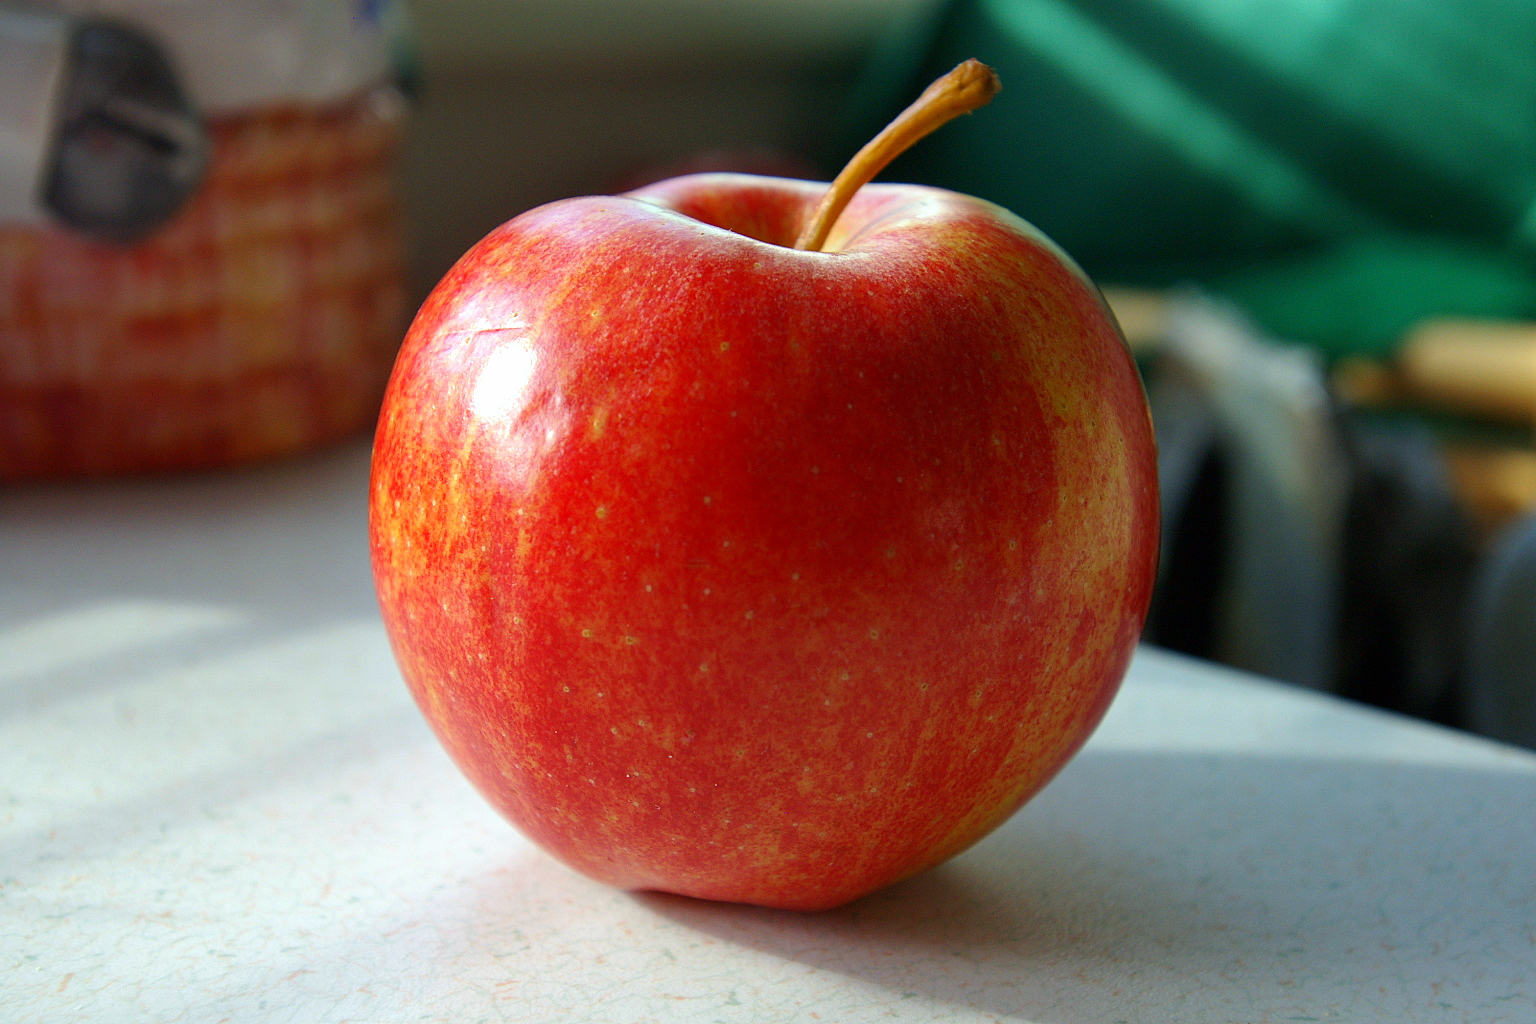
\includegraphics[width=0.60\linewidth]{manzana.jpg}
    \caption{Els científics i les científiques adoren comparacions com aquesta de la poma: permeten imaginar mides tan petites que el cervell, si només li dones metres, deixa de col·laborar. Imatge: Kim Siever, Wikimedia Commons, Public Domain.}
\end{figure}

Els àtoms no són estranys perquè siguin una ocurrència rebuscada. Són estranys perquè són a tot arreu i, tot i així, se'ns escapen contínuament. Són massa petits per veure'ls de la manera habitual i sovint només en percebem els efectes.

Per tant, la pregunta interessant no és tant ``podem veure un àtom?'', sinó una altra de molt millor:

\begin{center}
\textbf{Com sabem que és allà?}
\end{center}

La química podria començar just aquí. Sabem que hi ha alguna cosa sota el que veiem perquè deixa pistes pertot arreu. El joc consisteix a anar trobant aquestes pistes i comprovar si totes ens expliquen una història que tingui sentit.

Som-hi.

\section{Primera pista: l'aigua no regateja}

Comencem per una substància bastant poc sospitosa: l'aigua.

Sabem que és \ce{H2O}: dos àtoms d'hidrogen i un d'oxigen.

També coneixem aquell líquid que durant molts anys ha viscut als armariets de les farmacioles: l'aigua oxigenada. Si mirem l'etiqueta, hi apareix una altra fórmula: \ce{H2O2}.

Interessant.

\begin{center}
\ce{H2O} \qquad aigua

\ce{H2O2} \qquad peròxid d'hidrogen
\end{center}

La diferència sembla petita: hi hem afegit un oxigen. Però ja no és aigua. És una altra substància, d’aspecte molt semblant a l’aigua, però amb propietats diferents. I, si no, que t’ho diguin quan en cau una mica sobre una ferida. Potser aquests numerets ens estan intentant dir alguna cosa.

Recuperem ara la taula periòdica. Sí: resulta que no hi era únicament per obligar-nos a memoritzar caselles de colors. Si busquem les masses atòmiques aproximades, trobem:

\[
m_{\mathrm{H}}\approx 1\,\mathrm{u}
\qquad
m_{\mathrm{O}}\approx 16\,\mathrm{u}
\]

Són les masses aproximades d’un àtom de cadascun d’aquests elements, expressades en una unitat especial: la unitat de massa atòmica, o u. Aquesta unitat s’utilitza perquè els àtoms són tan petits que expressar-ne la massa en grams seria bastant poc pràctic.

Són masses extraordinàriament petites. Molt més petites que un gra de sorra. Molt més petites que una mota de pols de guix. Molt més petites del que probablement estàs imaginant ara mateix.

Ja veurem més endavant com dimonis podem conèixer una massa tan petita. De moment quedem-nos amb una idea: podem comparar les masses dels àtoms, i aquestes dades apareixen a la taula periòdica.

\begin{figure}[H]
    \centering
    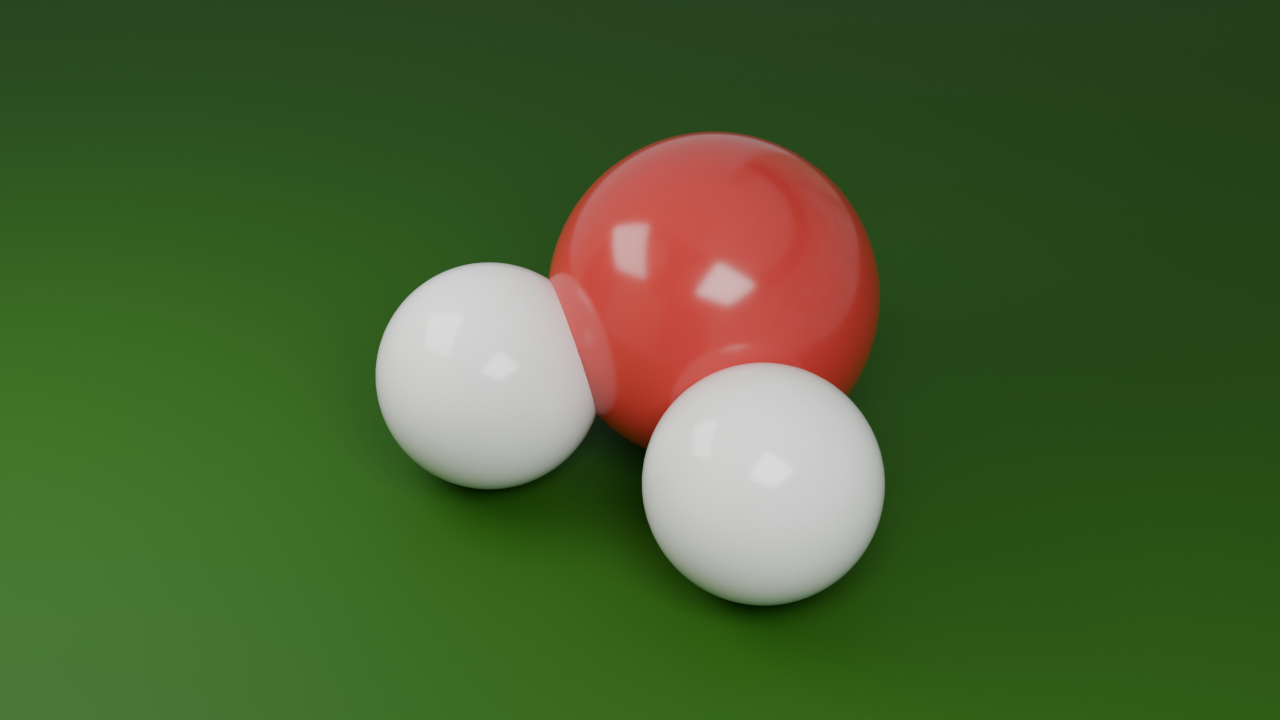
\includegraphics[width=0.60\linewidth]{molecula.png}
    \caption{Representació típica d’una molècula d’aigua, amb els seus tres àtoms convertits en boletes perquè alguna cosa hem de dibuixar. Les esferes representen aproximadament l’espai ocupat pels àtoms, i els colors segueixen una convenció habitual en química: oxigen en vermell i hidrogen en blanc. Imatge creada per l’autor, CC BY 4.0.}
\end{figure}

Si una molècula d'aigua conté dos hidrògens i un oxigen, la proporció de masses és:

\[
2\times 1 = 2
\qquad\text{i}\qquad
1\times16 = 16
\]

Per tant, per cada 2 parts de massa d'hidrogen en necessitem 16 d'oxigen.

Així, 2 g d'hidrogen poden combinar-se amb 16 g d'oxigen per formar 18 g d'aigua.

Què passa si tenim 20 g d'hidrogen però només 16 g d'oxigen?

No podem obligar l'aigua a portar més hidrogen perquè avui ens n'hagi sobrat. Els 16 g d'oxigen només poden reaccionar, en aquestes proporcions, amb 2 g d'hidrogen. La resta queda sense reaccionar.

És una mica com quan et sobra un ingredient d'un pastís i el guardes per a un altre dia. Només que aquí no podem decidir afegir-ne una mica més perquè quedi més dolç: \textbf{l'aigua té unes proporcions concretes i no negocia}.

I això no passa només amb l'aigua. Un compost químic pur presenta sempre la mateixa proporció entre els elements que el formen.

Això és la \textbf{llei de les proporcions definides}, associada sobretot al treball de Joseph Proust a finals del segle XVIII i començaments del XIX.

Ja tenim la primera pista.

\vfill
\newpage


\section{Segona pista: la natura sembla comptar}

No ens hem oblidat de l’aigua oxigenada. 

Si \ce{H2O} conté dos hidrògens i un oxigen, i \ce{H2O2} conté dos hidrògens i dos oxígens, gairebé podem imaginar que les estem construint amb peces.

Per una mateixa quantitat d'hidrogen, en un cas tenim una unitat d'oxigen i en l'altre en tenim dues. 
En massa passa el mateix:
\[
\ce{H2O}: 16 \text{ parts d'oxigen} + 2  \text{ parts d'hidrogen}
\]
\[
\ce{H2O2}: 32 \text{ parts d'oxigen} + 2  \text{ parts d'hidrogen}
\]

És a dir, amb aproximadament $16\ \mathrm{g}$ d'oxigen i $2\ \mathrm{g}$ d'hidrogen podem formar $18\ \mathrm{g}$ d'aigua.

En canvi, per formar peròxid d'hidrogen necessitem aproximadament $32\ \mathrm{g}$ d'oxigen i els mateixos $2\ \mathrm{g}$ d'hidrogen:
\[
32+2=34\ \mathrm{g}
\]

No obtenim una família contínua de compostos en què puguem anar afegint ``una mica'' d'oxigen fins a passar suaument de l'aigua al peròxid d'hidrogen. Les fórmules dels compostos estables apareixen amb nombres enters d'àtoms.

No trobaràs al botiquí un pot de \ce{H2O1.5}. A la farmàcia tampoc te'l donaran.

Així que en qualsevol dels dos casos ens sobra algun dels ingredients, aquesta part ja no pot entrar en aquella combinació. No desapareix ni s'improvisa una molècula nova: queda sense reaccionar i la podem guardar per a un altre dia.

\begin{quote}
Quan dos elements formen més d'un compost, les masses d'un d'ells que es combinen amb una mateixa massa de l'altre mantenen relacions senzilles de nombres enters.
\end{quote}


Això és la \textbf{llei de les proporcions múltiples}, formulada per John Dalton a començaments del segle XIX.

\vfill
\newpage

I torna a passar una cosa interessant: encara no hem vist cap àtom. Però la matèria es comporta com si estigués formada per peces.

I quan una cosa es comporta una vegada i una altra com si estigués feta de peces, comença a ser raonable sospitar que potser ho ho està.

\section{Dalton entra en escena}

Per aquí apareix John Dalton. Sí, sí: el mateix Dalton que anys més tard donaria classes al jove James Prescott Joule.

Dalton portava anys treballant amb gasos: mescles, pressions, expansió amb la temperatura i absorció de gasos en líquids. Cap al 1802--1803 va començar a explicar aquells comportaments suposant que la matèria estava formada per partícules últimes, diferents entre si i amb masses diferents.

Fins i tot va dibuixar símbols per representar els diferents àtoms i les seves combinacions. Avui aquells dibuixos ens poden semblar estranys, però la idea que hi havia darrere era potent: si la matèria està feta de peces, potser podem explicar les proporcions observades comptant-les.

\begin{figure}[H]
    \centering
    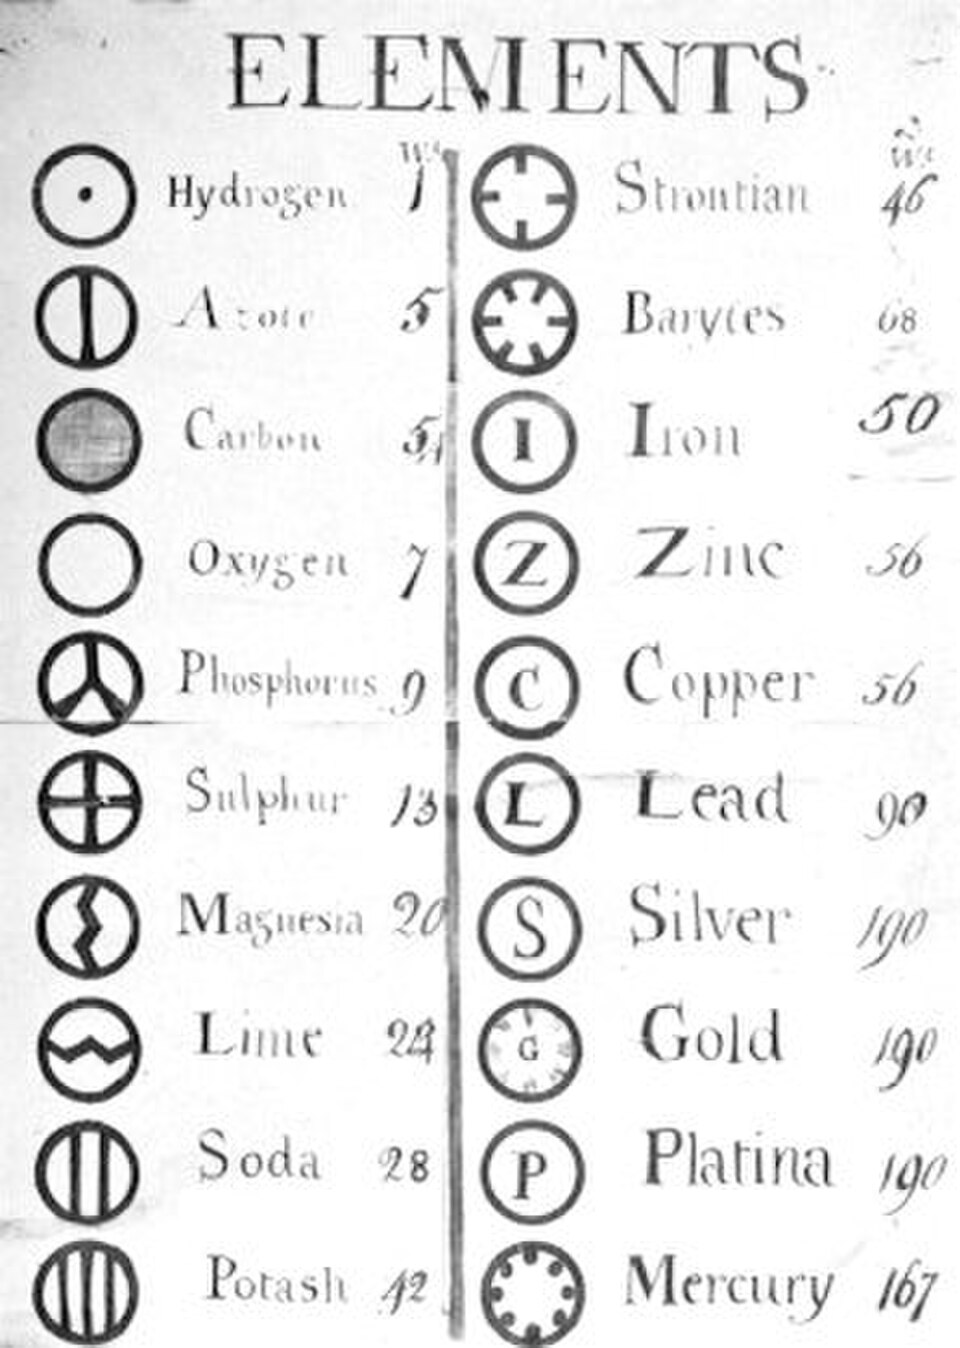
\includegraphics[width=0.60\linewidth]{dalton.jpg}
    \caption{Dalton va idear un símbol per representar cadascun dels elements coneguts a la seva època. També va intentar calcular la massa relativa dels seus àtoms i, tenint en compte els mitjans disponibles, en va obtenir alguns resultats sorprenentment bons. Wikimedia Commons, Public Domain.}
\end{figure}

La cosa pintava força bé. Però Dalton no estava treballant sol en un buit. Al seu voltant ja s'havien anat acumulant moltes altres pistas.

\subsection{Les evidències s’acumulen i això ja no hi ha qui ho pari.}

Fins ara, això és el que sabíem.

\begin{itemize}
    \item \textbf{Lavoisier} havia establert experimentalment que, en una reacció química ordinària, la massa total es conserva. Les substàncies canvien, però la matèria no desapareix perquè sí.

    \item \textbf{Proust} havia mostrat que un compost determinat conté els seus elements en proporcions de massa definides.

    \item \textbf{Dalton} va observar que, si dos elements formen diferents compostos, les quantitats que es combinen ho fan seguint relacions senzilles de nombres enters.
\end{itemize}

Mentrestant, a França estaven fent coses força divertides: posar gasos a reaccionar entre ells i mirar què passava. \textbf{Gay-Lussac} va trobar una altra regularitat: els volums que reaccionen també mantenen relacions senzilles. Dos volums per aquí, un per allà... una altra vegada apareixien nombres petits.

\begin{figure}[H]
    \centering
    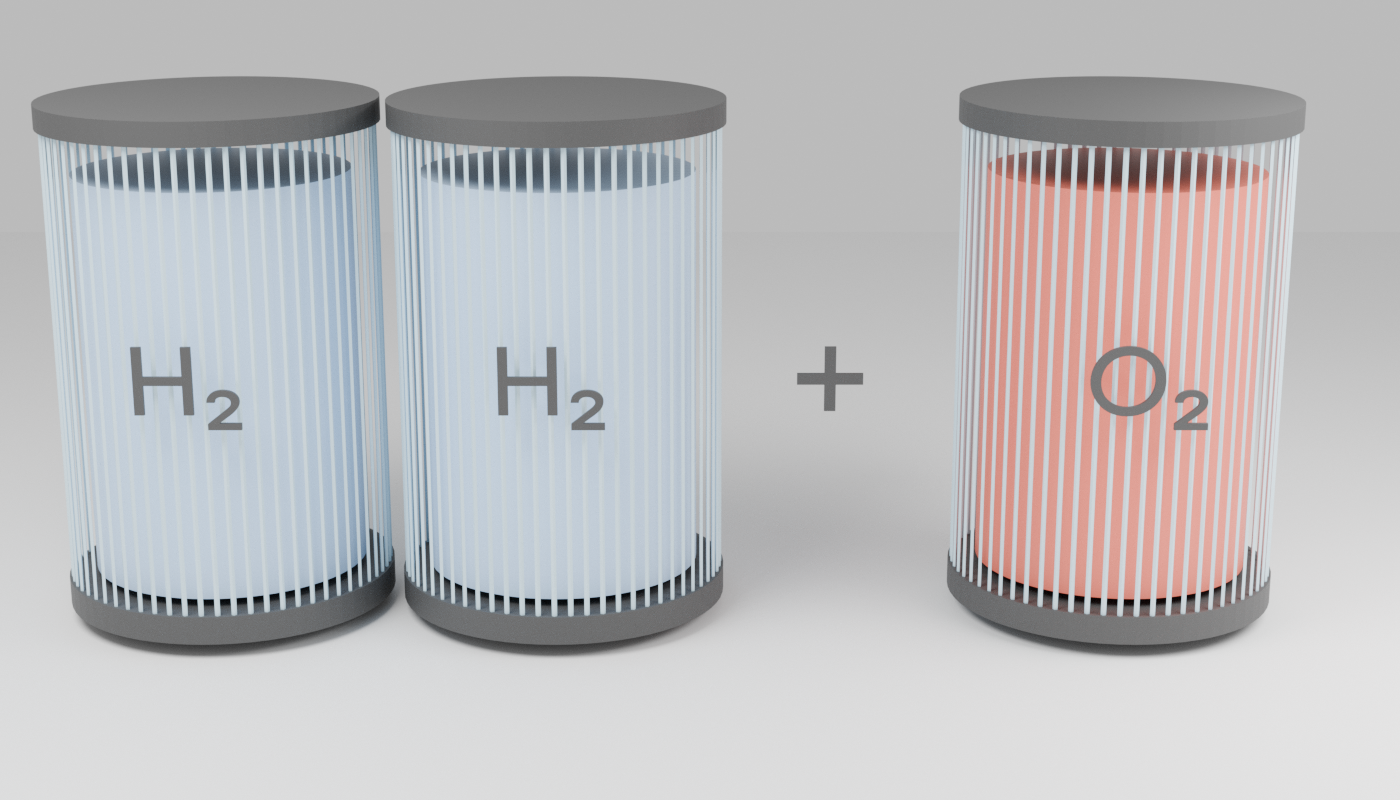
\includegraphics[width=0.60\linewidth]{volumenes.png}
    \caption{Dos volums d’hidrogen reaccionaven amb un volum d’oxigen per formar aigua, sempre parlant de gasos en les mateixes condicions de temperatura i pressió. A aquestes alçades ja s’estaven acumulant massa pistes per mirar cap a una altra banda. Imatge creada per l’autor, CC BY 4.0.. Imatge creada per l’autor, CC BY 4.0.}
\end{figure}

A Dalton, però, aquesta relació entre volums no li acabava d’agradar. El seu model funcionava força bé amb les proporcions de massa, però aquells nombres tan nets en els gasos no encaixaven fàcilment amb la manera com imaginava els àtoms i les seves combinacions.
La cosa començava a complicar-se. I, com passa sovint en ciència, quan les dades no encaixen amb el model, el problema acostuma a ser el model.

Què estava passant?

Cada experiment semblava diferent, però tots deixaven una mena de rastre comú: proporcions fixes, nombres enters, regularitats.

La natura semblava estar comptant coses.

\section{Avogadro posa una peça decisiva}

El 1811 va aparèixer Amedeo Avogadro.

Avogadro havia començat estudiant Dret. Però quan això de la física, la química i les matemàtiques et tira, de vegades et tira bastant fort.

La seva proposta era senzilla i molt potent:

\begin{center}
\textbf{Volums iguals de gasos, a la mateixa temperatura i pressió, contenen el mateix nombre de molècules.}
\end{center}

Aquesta hipòtesi ajudava a entendre per què els gasos reaccionaven en proporcions volumètriques tan simples.

I aquí la hipòtesi d’Avogadro encaixava especialment bé: explicava d’una manera sorprenentment elegant per què els gasos reaccionaven en proporcions de volum tan simples.

Si volums iguals contenen el mateix nombre de molècules, ja no estem barrejant quantitats misterioses, estem treballant amb quantitats proporcionals de partícules.

I apareixia, a més, una idea fonamental: les partícules d'un gas elemental podien estar formades per més d'un àtom. L'hidrogen podia existir com \ce{H2}, l'oxigen com \ce{O2}, i l'aigua podia ser \ce{H2O}.

De cop, moltes de les peces anteriors encaixaven en el mateix dibuix.

Això no significava que algú hagués vist un àtom.

Significava una cosa potser més interessant: \textbf{si suposàvem que els àtoms existien, molts experiments diferents deixaven de semblar casualitats i començaven a tenir sentit alhora}.

\vfill
\newpage


\section{I encara quedava molt per trencar}

A partir de Dalton, els àtoms ja servien per explicar força bé com es combinava la matèria. Però encara quedava una pregunta important: \textbf{eren realment indivisibles?}

Durant el segle XIX van aparèixer dues pistes que feien sospitar que la història era una mica més complicada.

La primera va arribar de la química. A mesura que es descobrien nous elements, van començar a aparèixer regularitats entre les seves propietats. Aquest ordre acabaria cristal·litzant en la taula periòdica. I la taula no era només una manera pràctica de posar cada element a la seva casella: el fet que certes propietats es repetissin indicava que, probablement, els àtoms tenien algun tipus d’estructura interna.

La segona pista va venir de l’electricitat. Els experiments mostraven que la matèria podia guanyar o perdre càrrega elèctrica i que, d’alguna manera, els àtoms hi estaven implicats. Si l’àtom podia perdre alguna cosa, potser aquella cosa havia de ser a dins.

Així, l’àtom de Dalton, aquella petita peça indivisible, va començar a deixar de semblar tan indivisible.

I és aquí on física i química comencen a mirar l’àtom de maneres una mica diferents. La química estudia sobretot com els àtoms s’uneixen, se separen i es reorganitzen per formar substàncies. La física, en canvi, començarà a preguntar-se \textbf{què hi ha dins de l’àtom}.

I com que un àtom no es pot obrir amb un tornavís, els físics van haver de buscar altres mètodes. Amb el temps, un dels més efectius seria accelerar partícules, estampar-les contra altres coses i mirar què surt. Una estratègia sorprenentment habitual en física.

Però ja tindrem temps de trencar àtoms.

De moment podem deixar descansar Dalton i companyia. Amb la idea que la matèria està formada per àtoms ja ens han fet avançar prou.

\section{Una última nota: Dalton no ho va encertar tot}

Hem simplificat algunes coses, perquè la història real de la ciència acostuma a ser una mica menys neta que el resum que fem després.

La teoria de Dalton explicava moltes observacions, però tenia algunes incomoditats que es van anar resolent amb el temps.

Dalton, per exemple, considerava que tots els àtoms d'un mateix element eren idèntics. Avui sabem que no és exactament així.

Existeixen els \textbf{isòtops}: àtoms d'un mateix element que tenen el mateix nombre de protons, però diferent nombre de neutrons. Per això continuen sent el mateix element, tot i que no tenen exactament la mateixa massa.

Químicament solen comportar-se de manera molt semblant perquè la química depèn sobretot de l'estructura electrònica, que per als isòtops d'un mateix element és gairebé la mateixa.

I Dalton també considerava l'àtom indivisible.

Això tampoc va durar.

Dins de l'àtom van aparèixer electrons, protons i neutrons, i després vam descobrir que alguns d'aquests components encara tenien més estructura.

Perquè quan la física troba una cosa que es diu ``indivisible'', sovint ho interpreta més aviat com una invitació.

Ja saps com va això: els químics fan servir els àtoms per construir molècules i substàncies noves; els físics els trenquen per veure què hi havia a dins.
